\documentclass[a4paper,addpoints,12pt]{exam}

\usepackage{dlds}
\usepackage{fig3d}
 
\begin{document}

\devoir[sem=2,prv=false,ds=false,num=6 ,niv=3 ,date=12/05/2023,Rdate=23/05/2023]

\begin{exo}
\begin{questions}
\question Soit $f$ une fonction linéaire et $(D)$ sa représentation graphique passe par le point $A(2;4)$.
\begin{parts}
\part Montrer que $f(x)=2x$.
\part Calculer $f(-3)$.
\end{parts}
\question Soit $g$ une fonction affine telle que $g(3)-g(-1)=-2$ et $g(0)=5$ et $(\Delta)$ sa représentation graphique.
\begin{parts}
\part Monter que $g(x)=-\dfrac{1}{2}x+5$.
\part Calculer $g(4)$.
\part Quel nombre a pour image -18 par $g$.
\end{parts}
\question Montrer que $(D)$ et $(\Delta)$ sont perpendiculaires.
\question Construire  $(D)$ et $(\Delta)$.
\end{questions}
\end{exo}

\begin{exo}
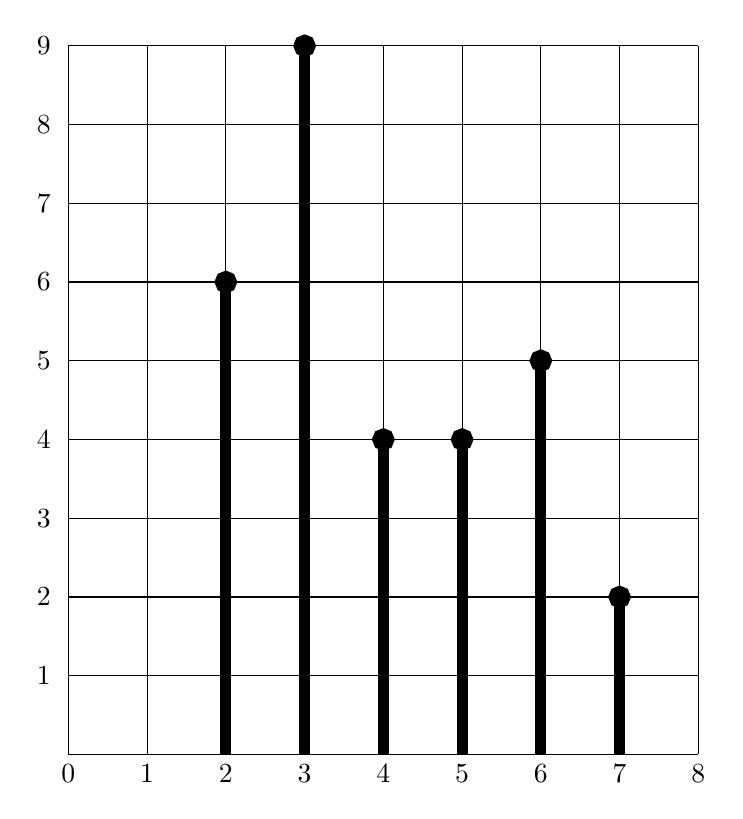
\begin{tikzpicture}
\draw (0,0) grid (8,9);
\foreach \y in {1,2,...,9} \draw(-0.1,\y)node[left]{\y};
\foreach \x in {0,1,...,8} \draw(\x,0)node[below]{\x};
\draw[line width=4pt] plot[ycomb,mark=*]  coordinates
{(2,6)(3,9)(4,4)(5,4)(6,5)(7,2)};
\end{tikzpicture}

Ce graphique représente les ventes des voitures d'une société durant les jours du mois du Juin.
\begin{questions}
\question Recopier et compléter le tableau suivant:
\begin{EnvFullwidth}
\begin{tabular}{|c|c|c|c|c|c|c|}
\hline 
Caractère & 2 & 3 & 4 & 5 & 6 & 7 \\ 
\hline 
Effectif &  &  &  &  &  &  \\ 
\hline 
Effectif cumulé  &  &  &  &  &  &  \\ 
\hline 
\end{tabular}
\end{EnvFullwidth}
\question Déterminer le mode de cette série statistique.
\question Calculer la moyenne des ventes par jours dans cette société.
\question Déterminer la médiane de cette série statistique. 
\end{questions}
\end{exo}

\begin{exo}
\begin{tikzpicture}
\cube[30]{3}{4}
\tkzDrawSegment(A,C)
\tkzDrawSegment(F,C)
\tkzDrawSegment[dashed](E,C)
\tkzDefPointOnLine[pos=0.5](A,C)\tkzGetPoint{I}
\tkzDefPointOnLine[pos=0.5](B,C)\tkzGetPoint{J}
\tkzDefPointOnLine[pos=0.5](C,F)\tkzGetPoint{K}
\tkzDefPointOnLine[pos=0.5](C,E)\tkzGetPoint{L}
\tkzDrawSegments(I,J J,K K,L L,I)
\tkzLabelPoint[below right=-4pt](I){I}
\tkzLabelPoint[below right=-4pt](J){J}
\tkzLabelPoint[below right=-2pt](K){K}
\tkzLabelPoint[below right=-4pt](L){L}
\end{tikzpicture}
Soit $ABCDEFGH$ un parallélépipède rectangle tel que $AB=4$ ; $AD=6$ et $AE=3$.
\begin{questions}
\question Calculer $EB$.
\question Montrer que $EBC$ est un triangle rectangle.
\question Calculer $EC$.
\question Déterminer le volume du pyramide $CEABF$.
\question La pyramide $CIJKL$ est une réduction de la pyramide $CEABF$ par le rapport $\dfrac{1}{2}$ 
\begin{parts}
\part Calculer $IJ$
\part Calculer le volume de la pyramide $CIJKL$.
\end{parts}
\end{questions}
\end{exo}
\end{document}